% ****** Start of file aipsamp.tex ******
%
%   This file is part of the AIP files in the AIP distribution for REVTeX 4.
%   Version 4.1 of REVTeX, October 2009
%
%   Copyright (c) 2009 American Institute of Physics.
%
%   See the AIP README file for restrictions and more information.
%
% TeX'ing this file requires that you have AMS-LaTeX 2.0 installed
% as well as the rest of the prerequisites for REVTeX 4.1
% 
% It also requires running BibTeX. The commands are as follows:
%
%  1)  latex  aipsamp
%  2)  bibtex aipsamp
%  3)  latex  aipsamp
%  4)  latex  aipsamp
%
% Use this file as a source of example code for your aip document.
% Use the file aiptemplate.tex as a template for your document.
\documentclass[%
 aip,
% jmp,
% bmf,
% sd,
% rsi,
 amsmath,amssymb,
%preprint,%
 reprint,%
%author-year,%
%author-numerical,%
% Conference Proceedings
]{revtex4-1}

\usepackage{graphicx}% Include figure files
\usepackage{dcolumn}% Align table columns on decimal point
\usepackage{bm}% bold math
%\usepackage[mathlines]{lineno}% Enable numbering of text and display math
%\linenumbers\relax % Commence numbering lines

\usepackage[utf8]{inputenc}
\usepackage[T1]{fontenc}
\usepackage{mathptmx}

\begin{document}

\preprint{AIP/123-QED}

\title{A GEM-based Optically Readout Time Projection Chamber for charged particle tracking}
% Force line breaks with \\
 \author{V. C. Antochi}\altaffiliation[Also at ]{Dipartimento di Fisica Sapienza Universit\`a di Roma, I-00185, Italy now at Oskar
 Klein Centre, Department of Physics, Stockholm University, AlbaNova, Stockholm SE-10691, Sweden}
\author{G. Cavoto}\altaffiliation[Also at ]{Dipartimento di Fisica Sapienza Universit\`a di Roma, I-00185, Italy}
\author{I. A. Costa}\altaffiliation[Also at ]{Universidade Federal de Juiz de Fora, Juiz de Fora, MG, Brazil}
\author{E. Di Marco}
\author{G. D'Imperio}
\author{F. Iacoangeli}
\author{M. Marafini}\altaffiliation[Also at ]{Museo Storico della Fisica e Centro Studi e Ricerche "Enrico Fermi" Piazza del Viminale 1, Roma, I-00184, Italy}
\author{A. Messina}\altaffiliation[Also at ]{Dipartimento di Fisica Sapienza Universit\`a di Roma, I-00185, Italy}
\author{D. Pinci}
\author{F. Renga}
\author{C. Voena}
\affiliation{Istituto~Nazionale~di~Fisica~Nucleare
Sezione di Roma, I-00185, Italy}

 \author{E. Baracchini}
 \author{A. Cortez}
 \author{G. Dho}
 \altaffiliation[Also at ]{Istituto Nazionale di Fisica Nucleare, Laboratori Nazionali del Gran Sasso, Assergi, I-67100, Italy}
 \affiliation{Gran~Sasso~Science~Institute~L'Aquila, I-67100, Italy}
\author{L. Benussi}
\author{S. Bianco}
\author{C. Capoccia}
\author{M. Caponero}\altaffiliation[Also at ]{ENEA Centro Ricerche Frascati, Frascati, I-00044, Italy}
\author{G. Maccarrone}
\author{G. Mazzitelli}
\author{A. Orlandi}
\author{E. Paoletti}
\author{L. Passamonti}
\author{D Piccolo}
\author{D Pierluigi}
\author{F. Rosatelli}
\author{A. Russo}
\author{G. Saviano}\altaffiliation[Also at ]{Dipartimento di Ingegneria Chimica, Materiali e Ambiente, Sapienza Universit\`a di Roma, Roma, I-00185, Italy}
\author{S Tomassini}
\affiliation{Istituto Nazionale di Fisica Nucleare
Laboratori Nazionali di Frascati, I-00040, Italy}

\author{R. A. Nóbrega}\affiliation{Universidade Federal de Juiz de Fora, Juiz de Fora, MG, 36000-000, Brazil}

\author{F Petrucci}\altaffiliation[Also at ]{Istituto Nazionale di Fisica Nucleare, Sezione di Roma TRE, Roma, I-00146, Italy}

\affiliation{Dipartimento di Matematica e Fisica, Universit\`a Roma TRE, Roma, I-00146, Italy}




%% \author{A. Author}
%%  \altaffiliation[Also at ]{Physics Department, XYZ University.}%Lines break %% automatically or can be forced with \\
%% \author{B. Author}%
%%  \email{Second.Author@institution.edu.}
%% \affiliation{ 
%% Authors' institution and/or address%\\This line break forced with %% \textbackslash\textbackslash
%% }%
%% 
%% \author{C. Author}
%%  \homepage{http://www.Second.institution.edu/~Charlie.Author.}
%% \affiliation{%
%% Second institution and/or address%\\This line break forced% with \\
%% }%

\date{\today}% It is always \today, today,
             %  but any date may be explicitly specified

\begin{abstract}
The Time Projection Chamber (TPC) is an ideal candidate to track  particles in a wide range of energies. Large volumes TPCs  can be readout with a suitable number of channels offering a complete 3D reconstruction of the charged particle tracks and of their  released energy  allowing the  identification of their mass. Moreover, He-based TPC's  are very promising  to study keV  energy particles, opening the possibility for directional searches  of Dark Matter (DM)  and the study of Solar Neutrinos (SN). On the other hand, in order to reach a keV energy threshold, a large number of channels is required to obtain a high granularity, that could be expensive and hard to manage.

A small prototype (named LEMOn) to test and validate an innovative read-out technique is described here. It based on the amplification of the ionization in Micro Pattern Gas Detector (MPGD) producing visible light collected by a sub-millimeter position resolution sCMOS (scientific CMOS) camera. This type of readout - in conjunction with a fast light detection - allows a 3D reconstruction of the tracks, a  sensitivity to the track direction and a very promising  particle identification capability useful to distinguish  DM nuclear recoils from a $\gamma$-induced  background.
\end{abstract}

\maketitle

%% \begin{quotation}
%% The ``lead paragraph'' is encapsulated with the \LaTeX\ 
%% \verb+quotation+ environment and is formatted as a single %% paragraph before the first section heading. 
%% (The \verb+quotation+ environment reverts to its usual %% meaning after the first sectioning command.) 
%% Note that numbered references are allowed in the lead %% paragraph.
%% %
%% The lead paragraph will only be found in an article being %% prepared for the journal \textit{Chaos}.
%% \end{quotation}
%%
\begin{quotation}

Large Time Projection Chambers (TPC)  have various applications in high energy physics and nuclear physics. These detectors are among the best in  offering good charged particle  energy resolution and to allow the identification of the  particle's mass. This can be obtained along with a very good performance in tracking the particle's  trajectory  with competitive spatial resolution.
The study of such a technology for ultra-rare events searches as the directional search of  Dark Matter \cite{Battat:2016xxe, Battat:2016pap, Battat:2014van} (DM) and the detection of neutrinos coming from the Sun (SN) \cite{Seguinot:1992zu, ARPESELLA1996333} is currently being pursued by several groups, which are part of the CYGNUS\cite{CYGNUSweb} international network\cite{baracchini2019cygno}.

  A longer term project for tens of m$^3$ volume TPC requires the construction of 1 m$^3$ demonstrators. In this paper we describe the  performance of a smaller 7 litres prototype (named LEMOn) in tracking ultra-relativistic electrons. LEMOn is based on Micro Pattern Gaseous Detectors (MPGD), namely a large triple Gas Electron Multiplier (GEM)\cite{Sauli:1997qp}, optically read-out by means of a low noise and high granularity sCMOS sensor\cite{ bib:jinst_orange1, bib:nim_orange2}.

Many smaller scale prototypes have been tested so far showing promising results to design the CYGNO 1 m$^3$ demonstrator to be constructed in  2020-2021 and to be hosted at the INFN  National Laboratory of Gran Sasso (LNGS). In a later phase, a 30-100 m$^3$ detector is foreseen, as a brick of a world distributed observatory for DM and SN within the CYGNUS international network.  
\end{quotation}
\section{Introduction}
The purpose of the current R\&D phase is to asses the performance  of a relatively large TPC based on the drift of the  ionization electrons   within a He-based gas mixture operated at atmospheric pressure and  equipped with a high granularity and high sensitivity optical readout of GEMs. In this respect the test of the LEMOn prototype  with ultra-relativistic electrons presented here  is meant to study the capability of the optically readout TPC to detect   and to reconstruct within the TPC drift region  the positions of clusters with few  ionization electrons each. The pattern of contiguous clusters represents the "track" of the ultra-relativistic electron trajectory and are exploited to  identify  it,  demonstrating that LEMOn  would also be an excellent beam monitoring device.

 In absence of a reference time for the events, electron drift time can not be exploited to extract information about their depth inside the detector. In this paper, we study a method to measure the  longitudinal position of an ionizing particle in the TPC drift volume based on the electron diffusion and therefore without relying on the time of the particle interaction in the gas which is unknown in DM search. It helps  to fully define a fiducial gas volume, so that background events  generated by the detector components, in particular the cathode and the amplification system (as the GEMs), can  be discarded.
 
The MPGD optical readout can in fact  represent a change in the paradigm of TPCs for rare events searches:
\begin{itemize}
\item optical sensors offer higher granularity with respect to electron sensitive devices;
\item optical coupling allows to keep the sensors out of the sensitive volume, reducing the interference with the high
voltage operation and  the gas contamination;
\item the use of suitable lenses enables the imaging of  large surfaces to small sensors.
\end{itemize}
Moreover, in last years, optical sensors market had an impressive development: sensors able to provide the required large granularity along with a very low noise level and high sensitivity to single photon counting are now available.

Recently, many  tests have been conducted  with different prototypes (NITEC~\cite{JINST:nitec}, ORANGE~\cite{NIM:Marafinietal, bib:jinst_orange2}, LEMOn~\cite{bib:eps, bib:ieee17, bib:elba}) with various particles sources (electron beam test facility, neutron beams and  different radioactive sources). In the following, we report the results obtained with the LEMOn prototype at the Frascati Beam Test Facility (BTF).


\section{LEMOn Prototype Design}

The LEMOn prototype structure (Fig. \ref{fig:sex}) was made of  ASA, Acrylonitrile Styrene Acrylate, at the 3D printing Facility of the National Laboratory of Frascati (LNF)\cite{3dprinting} of INFN. This has offered the opportunity  to easily design and to quickly develop detectors and also to test the 3D printing system for gas detector applications.


The LEMOn's heart consists of a 7 liter active drift volume surrounded by a  200$\times$240~mm$^2$ elliptical field cage with a 200 mm distance between the anode and the cathode. The electric field is  shaped by  1~mm Cu+Ag wires held at their positions  by nineteen 3D-printed rings. The anode side is instrumented with a 200$\times$240~mm$^2$ rectangular triple  GEM structure located at a position 10 mm apart from the last field cage ring. They are LHCb-like \cite{bib:thesis}  GEMs  with 70~$\mu$m diameter holes and 140~$\mu$m pitch   and  with two 2 mm wide  transfer  field gaps among them (Fig.~\ref{fig:gem}).  A $203\times254\times1$ mm$^3$ transparent window 
and a  bellow with a tunable length allow  to collect the light emitted from the GEMs by using an ORCA-Flash 4.0 camera \cite{ORCAcamera}. This camera is positioned  at a 52 cm  distance from the outemost  GEM layer and is based on a sCMOS sensor with a high granularity ($2048\times2048$ pixels), very low noise (around two photons per pixel), high sensitivity (70\%  quantum efficiency at  600~nm) and good linearity. This camera is instrumented with a Schneider lens (f/0.95-25~mm ). The lens is placed at a distance $d$ of 50.6 cm from the last GEM
in order to obtain a de-magnification
$\delta = (d/f) - 1 = 19.25$ to
image a surface $25.6 \times 25.6$~cm$^2$ onto the
$1.33 \times 1.33$~cm$^2$ sensor.
In this configuration, each pixel
 is therefore imaging  an effective area of 125$\times$125~$\mu$m$^2$ of the GEM layer. The fraction of the light collected by the lens can be evaluated \cite{bib:jinst_orange1} to be $1.7 \times 10^{-4}$.

\begin{figure}[!ht]
\centering
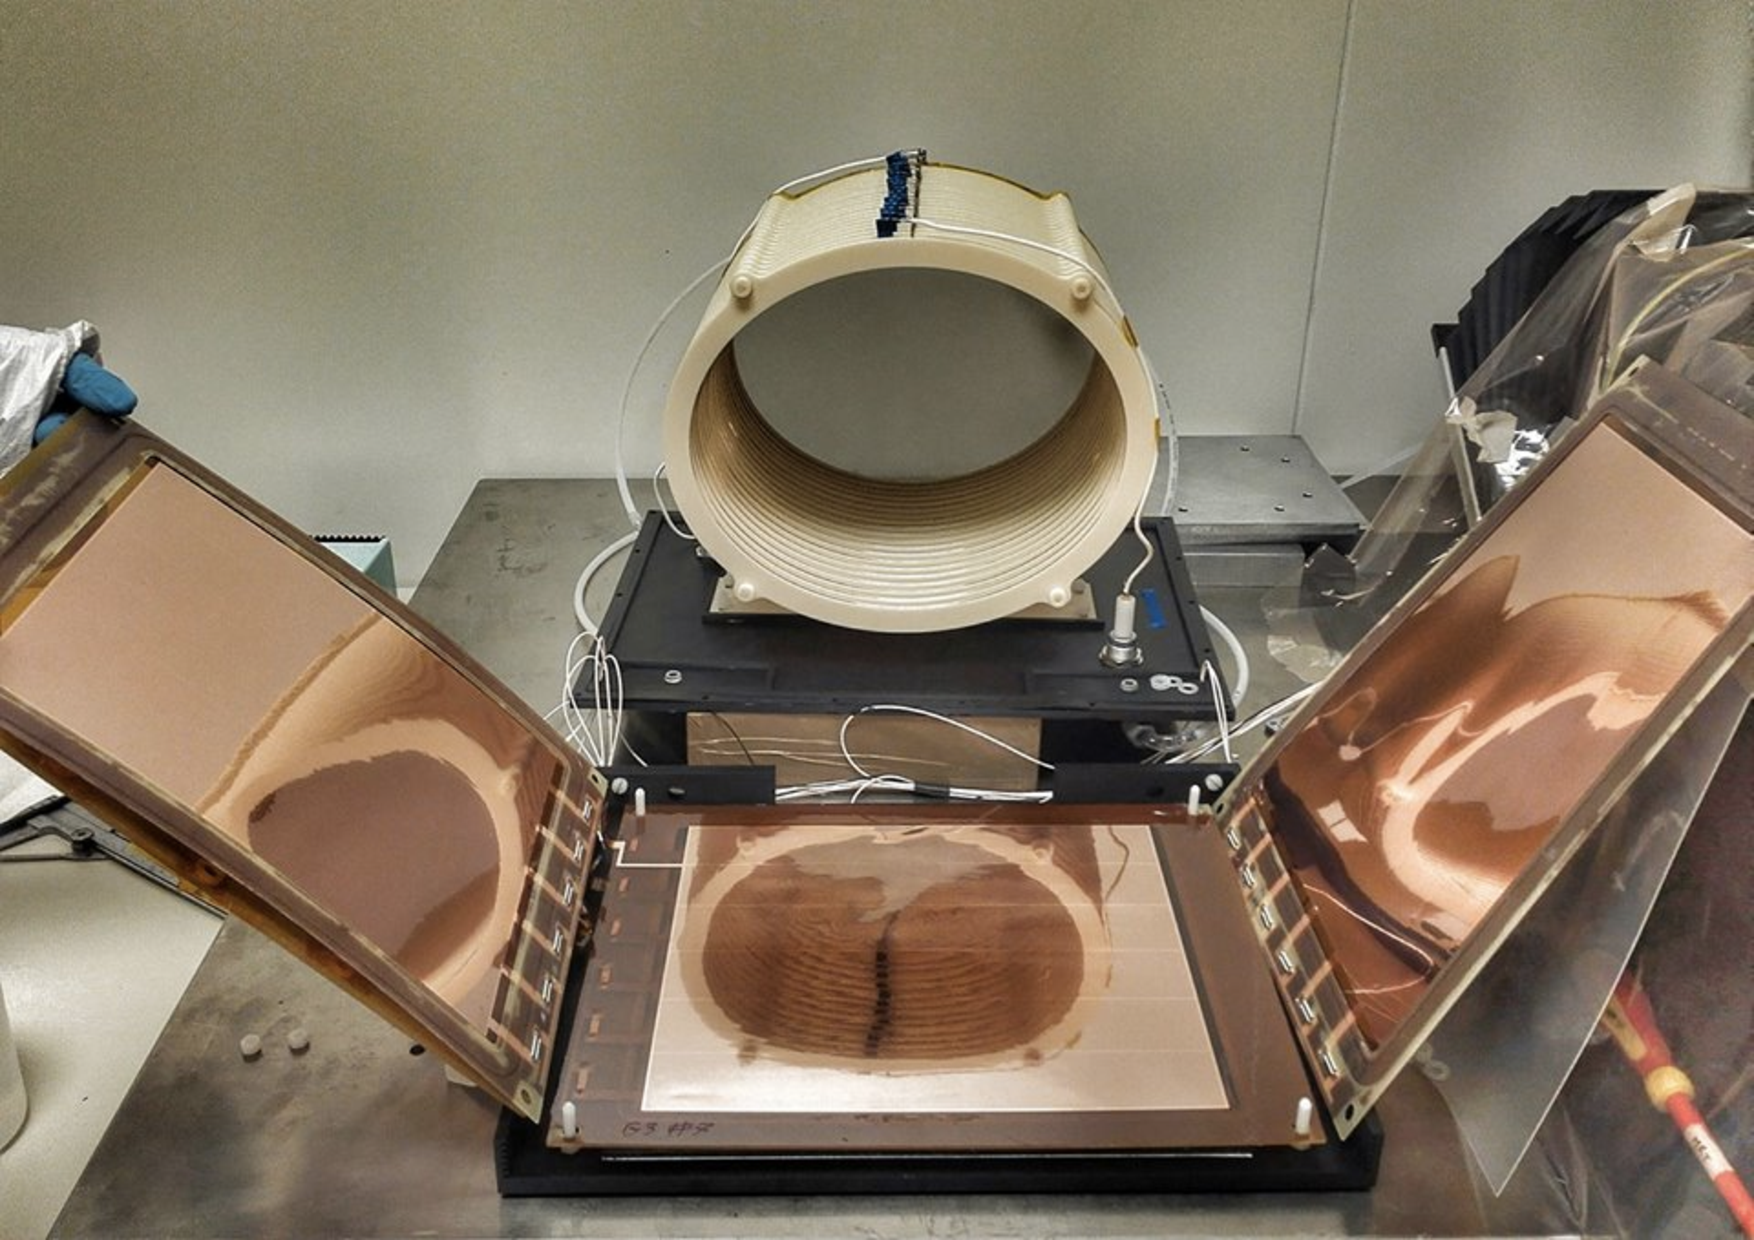
\includegraphics[scale=0.290]{Fig1-gem.pdf}\DeclareGraphicsExtensions.
\caption{Exploded triple GEM structure (on the front)  with  the 3D-printed field cage rings (white)  equipped with a semi-transparency cathode (on the back of the rings).}
\label{fig:gem}
\end{figure}

On the cathode side, LEMOn has been equipped with a 50$\times$50~mm$^2$ HZC Photonics XP3392 photomultiplier \cite{PMTPhotonics} (PMT) detecting light through a transparent $50\times50\times4$~mm$^3$ fused silica window.
\begin{figure*}[!ht]
\centering
 \framebox{\parbox{6.7in}{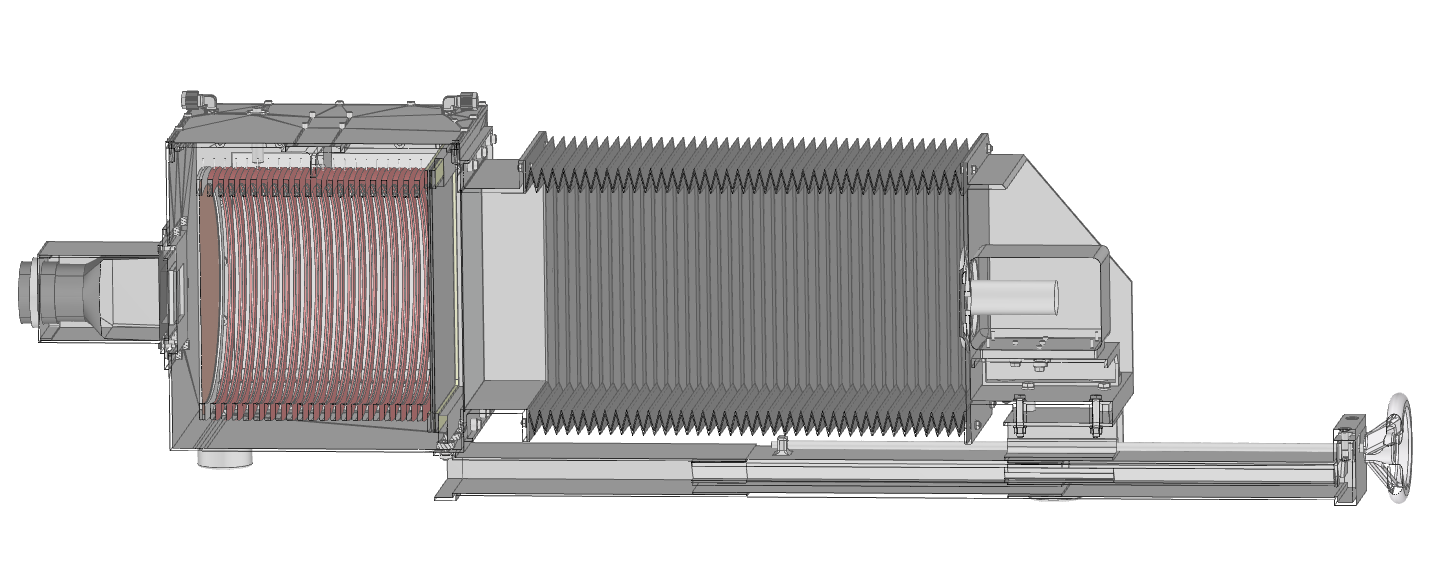
\includegraphics[width=1\linewidth]{Fig2-section.png}}}
\caption{LEMOn 3D printing design. From the left to the right:  PMT holder, semi-transparent cathode, field cage rings (in red),  the triple GEM stack,a large transparent window, the optical  bellow and the  ORCA Flash camera holder.}
\label{fig:sex}
\end{figure*}

This PMT  also allowed to study - mainly for timing purpose -  the primary scintillation light emitted   in the drift volume by the BTF electrons themselves and the secondary light produced by the innermost GEM layer 200 mm far away during the development of the electron avalanche. A  cathode has been realized using an ATLAS MicroMegas mesh, produced
by Swiss BOOP company, stretched and glued on ring, 1 cm apart from the last ring of the field cage and ensuring an adequate light transmission. Its transparency to light has been estimated to be about $70\%$. The  field cage is contained in a  $370\times270\times280$~mm$^3$ and 2.5~mm thick box. This box has been equipped with two 180~$\mu$m thin $200\times200$~mm$^2$ windows made of TEDLAR in order to guarantee the gas containment and to reduce as much as possible the multiple scattering of the impinging ultra-relativistic  electrons (or the absorption of other particles).

\section{Detector Operations}

The data reported in this paper have been collected at the Frascati Beam Test Facility~\cite{bib:btf} which can deliver bunched electrons or positrons from few tens of MeV to several hundred MeV energy. The BTF is optimized to deliver electrons with an energy of 450 MeV with  a typical beam spot size of $\sigma_{x,y}\simeq$~2~mm, a divergence  $\sigma^\prime_{x,y}\simeq$~2~mrad, and an energy spread of $\simeq$~1\%. Moreover, for our measurements the bunch multiplicity has been tuned to be  single particle, with the possibility to change it up to several hundred  electrons (with 10~ns bunch length). The bunch multiplicity and the beam spot-size were monitored by means of a Fitpix \cite{Kraus_2011} detector located upstream of LEMOn  and a Pb-glass  calorimeter~\cite{Buonomo:2017sdz} ~\cite{Buonomo:2017btf} accommodated at the back of LEMOn and acquired in coincidence with  the LEMOn camera image and the  PMT signal. 

\begin{figure}[!ht]
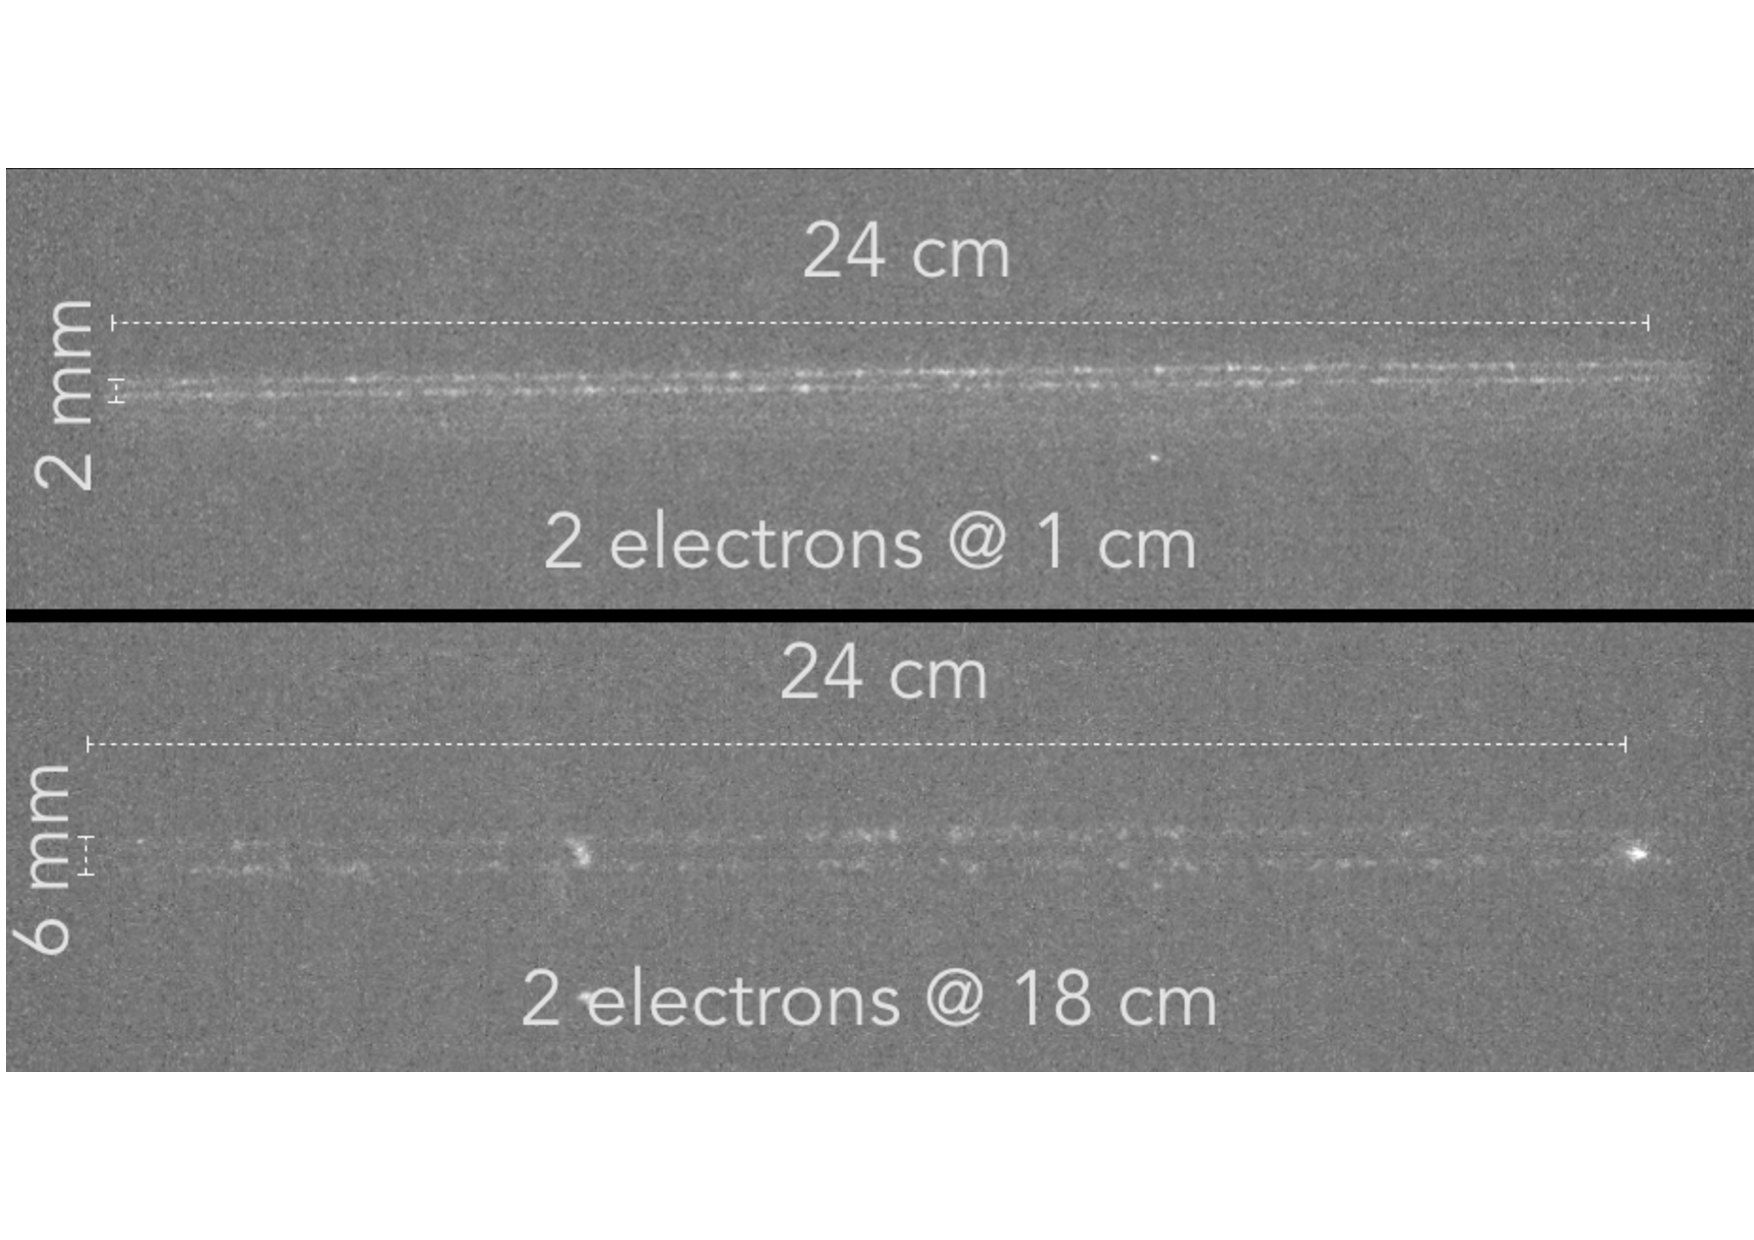
\includegraphics[width=3in]{Fig3-tracks.pdf}\DeclareGraphicsExtensions.
\caption{Two examples of  two-tracks events collected at the Frascati BTF. The two BTF electrons are crossing the field cage parallel  to  the  240~mm major axis. One event is acquired with the beam   close to the GEM (up), and another with the beam 180 mm far away  from the GEM (down). The separation among the two track can be easily measured.}
\label{fig:track}
\end{figure}

LEMOn was operated at BTF with a He-CF$_4$ (60/40) gas mixture, the triple GEM system set at a voltage across the GEM sides of 455~V and an electric field between them of 2.0 kV/cm. The gas mixture was kept at atmospheric pressure under continuous flow of about 100 cc/min and with the GEMs operated  at very high gain ($> 5\times10^5$) in order to reach a good light production in  the avalanche generated in the  GEMs structure. The typical photon yield for this  type of gas mixtures has been measured to be around  0.07 photons per avalanche electron.\cite{bib:jinst_orange1, bib:roby, bib:tesinatalia}

The field cage was powered by a CAEN N1570.\cite{CAENN1570} This posed a limitation to    the maximum  electric field  at 0.6 kV/cm. 

Some data has also been collected at a lower field in order to study the field cage performance. The triple GEM system was powered with a HV GEM power supply \cite{Corradi:2007df} ensuring stability and accurate monitoring of the bias currents.

The ORCA Camera I/O has been configured in order to get a pre-trigger, that must occur 80~$\mu$s before the shutter, and to synchronize the PMT signal waveform acquired with an oscilloscope LeCroy 610Zi. Optics and exposure time (30~ms) were optimized to ensure the largest light collection and to avoid events due to the natural radioactivity. Between 100 and 300 images were typically acquired per run. 
Fig.~\ref{fig:track} shows two examples of BTF electron tracks images acquired with LEMOn.

The 450 MeV  BTF  electrons were delivered by the LNF accelerator complex  along the X axis direction (see Fig.\ref{fig:frame})  with a repetition rate of one bunch every  second. LEMOn was accommodated over a remotely controlled table  in order to scan  the $Y$ and $Z$ coordinates (with a 0.2 mm precision). 

\begin{figure}[!ht]
\centering
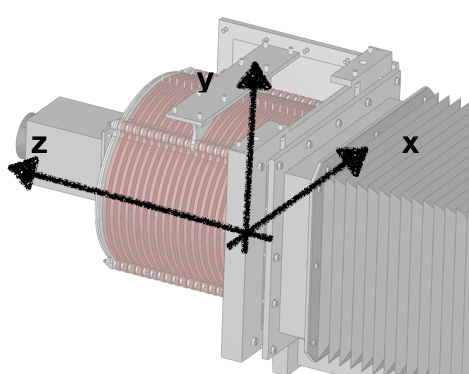
\includegraphics[width=3in]{Fig4-referenceFrame.png}\DeclareGraphicsExtensions.
\caption{Reference frame: the origin of the axis is located at the middle of the GEM plane in vertical Y coordinate, while the X origin is located at the beginning of the GEM plane to coincide with the particle track length; moreover, the Z coordinate represents the distance from the GEM plane starting from it}
\label{fig:frame}
\end{figure}


\section{Test Beam Results}

Data were collected at the LNF BTF during a week long campaign, when LEMOn was continuously operated. 

The fast PMT signal waveform was acquired using as external trigger from the timing signal of the BTF line synchronized with the electrons arrivals. The time $t_{s}$ corresponding to a fixed voltage of the PMT waveform was associated to each PMT signal and data at different longitudinal $Z$ position were collected. 
The standard deviation ($SD_t$) of the distribution of the residuals of $t_{s}$ at each $Z$ can be converted into the standard deviation ($SD_Z$) of the BTF electrons $Z$ position using the gas mixture drift velocity. A value of $SD_Z$ around  1 mm  was found,  well compatible with the  beam spot transverse size. 

Each image acquired with the sCMOS camera was saved as a 2048 x 2048 matrix of photon counts. 
 Because of the very low occupancy of sensor, the baseline noise of the sensor is estimated pixel by pixel by obtaining the distribution of counts for each pixel in all the images of a data-taking run. The  average count and the standard deviation ($\sigma_n$) for each pixel is then evaluated. This average photon count  is subtracted to the count of each image before the image is further processed. 
 
 The reconstruction  of tracks in each image is then made by using a Hough transform pattern recognition algorithm (HT) \cite{bib:hough}. Since LEMOn is positioned to let the BTF electrons cross the drift volume at $Y$ $\sim$ 0, only pixels with a photon count exceeding 1.5$\sigma_n$ are used in the HT. The HT could finds several lines connecting all the pixels above this threshold: the most ranked line within an angle of about $\pm 5$ mrad respect to the $X$ axis is then selected in each image and it represents the candidate reconstructed BTF electron (a {\it track}). Multiple track images are also analyzed and the HT is in fact able to distinguish  tracks in events with multiplicity larger than one.
 
The efficiency to reconstruct a BTF electron crossing the 24 cm wide drift region it is measured to be very close to unit. In fact, a Garfield \cite{bib:garfield1, bib:garfield} simulation of the  gas mixture yields an  estimate for the  average  energy loss of 0.20 keV/mm for a  $\simeq$~450 MeV electron. This energy loss translates into three primary ionization e$^-$ cluster per mm. The sequence of several ionization clusters along the BTF electron trajectory is in fact a clear signature to detect each BTF electron. 
We check this prediction by selecting in the runs the events with a Pb-glass calorimeter signal compatible with a single BTF  electron  deposit. In these events  we always find a BTF track in the  sCMOS image.

\subsection{Tracking performances}

 
 The total light  yield distribution transverse to the track direction is obtained for each track (Fig. \ref{fig:tracking}). This distribution is fitted to a Gaussian function  and its integral  is  proportional to the total energy loss of the track in the gas volume of the field cage. 
 
\begin{figure}[!ht]
\centering
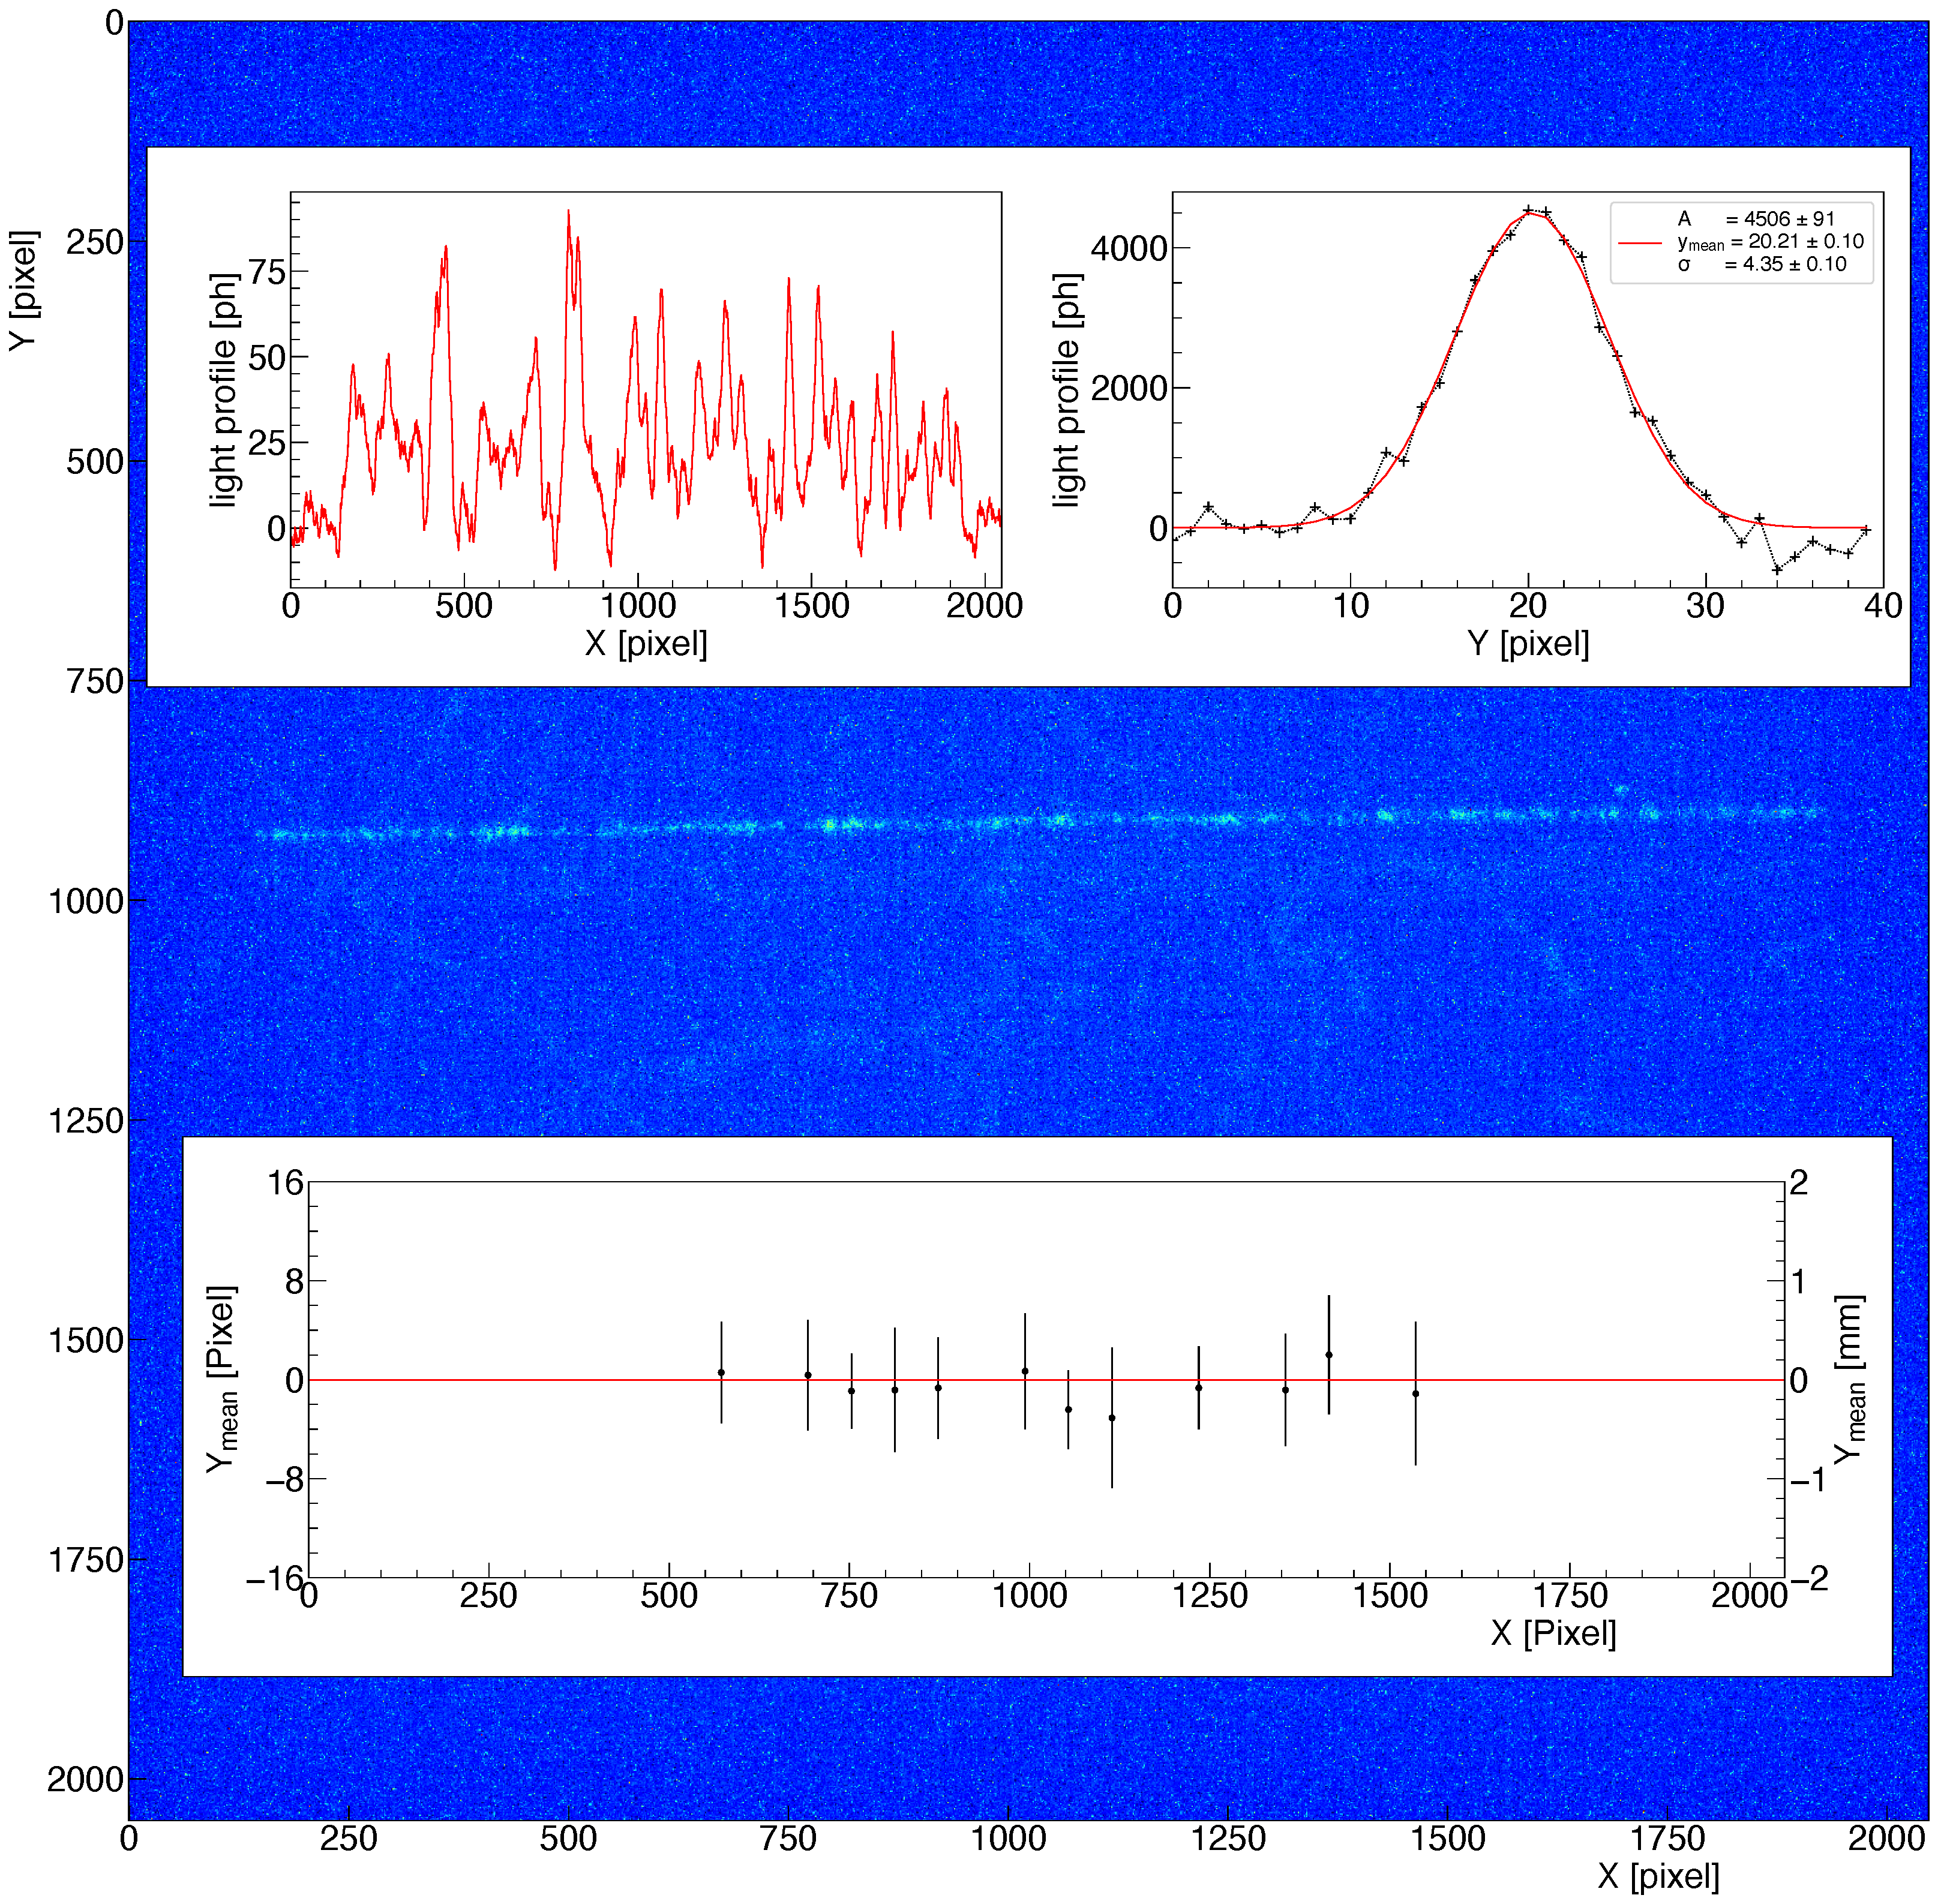
\includegraphics[width=3.4in]{Fig5-Track-Z.pdf}\DeclareGraphicsExtensions.
\caption{{\bf Background}: sCMOS camera  image collected at the LNF BTF 6.5 cm apart from GEM plane, pixels with a number of counts larger than the average noise and due to a BTF electron are visible at $Y$ $\sim$ 1000. {\bf Left top insert}:  light distribution (after pixel-by-pixel noise subtraction) along the track $X$-direction summing all the photons for 40 pixel in the  $Y$ direction around the track direction. {\bf Right top insert}:    light distribution  transverse to the track ($Y$ direction) summing all the photons along the  $X$ direction  with a superimposed Gaussian fit. {\bf Bottom insert}: Gaussian $Y_{mean}$ of the transverse light distribution for each of the 18 segments with  the line found by the HT. The error bar of the points is the sigma of the normal fit in each slice and it is taken as a indication of the width of the light deposit. Some segments with a  too low signal-to-noise ratio of the detected light are not displayed. }
\label{fig:tracking}
\end{figure}


 In different runs the LEMOn position along $Z$ is changed resulting in a different $Z$ coordinate for the tracks. These runs  are used to evaluate the uniformity of the response across the field cage. The total light yield  per track is in fact  fairly uniform,  with a slight decrease at  $Z$ positions farther away  from the GEMs (see Fig.\ref{fig:lightvsZ}). This is likely due to the electron attachment to gas impurities during the drift of  the ionization electrons from their production points along the track to the GEMs.
  Moreover, the relative fluctuation of the total light yield per track represents an estimate of the energy loss resolution of LEMOn (Fig.\ref{fig:energyresvsZ}). This turns out to be about 20\% and almost independent on the $Z$ position of the track.
 
 \begin{figure}[!ht]
\centering
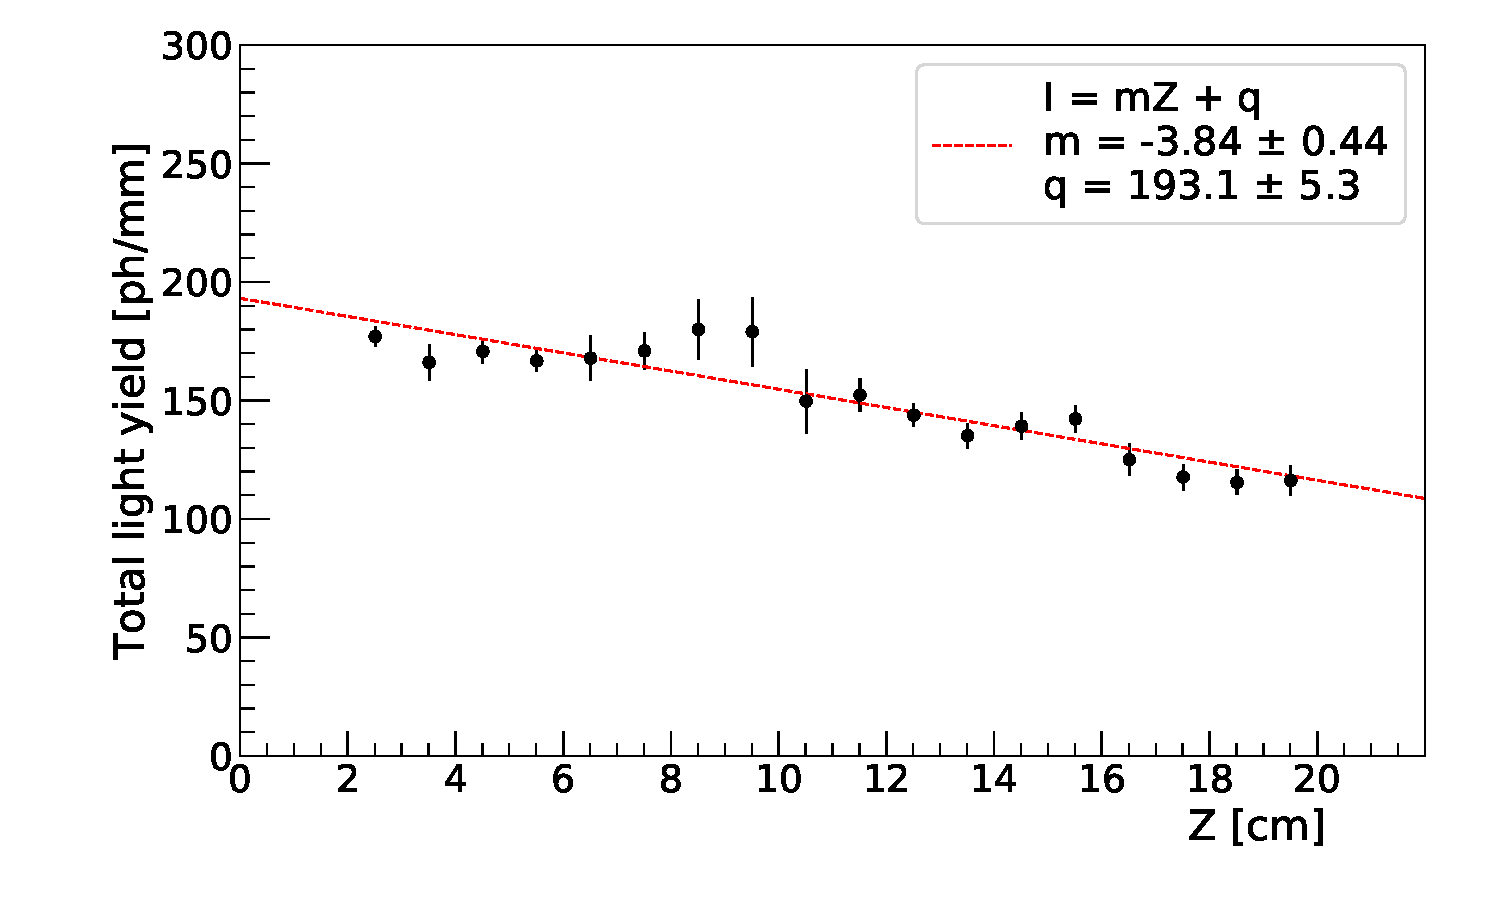
\includegraphics[width=3.4in]{Fig6-Photons-Z.pdf}
\caption{Average total light yield $I$ per track as a function of the track $Z$ position across the field cage.}
\label{fig:lightvsZ}
\end{figure}

  \begin{figure}[!ht]
\centering
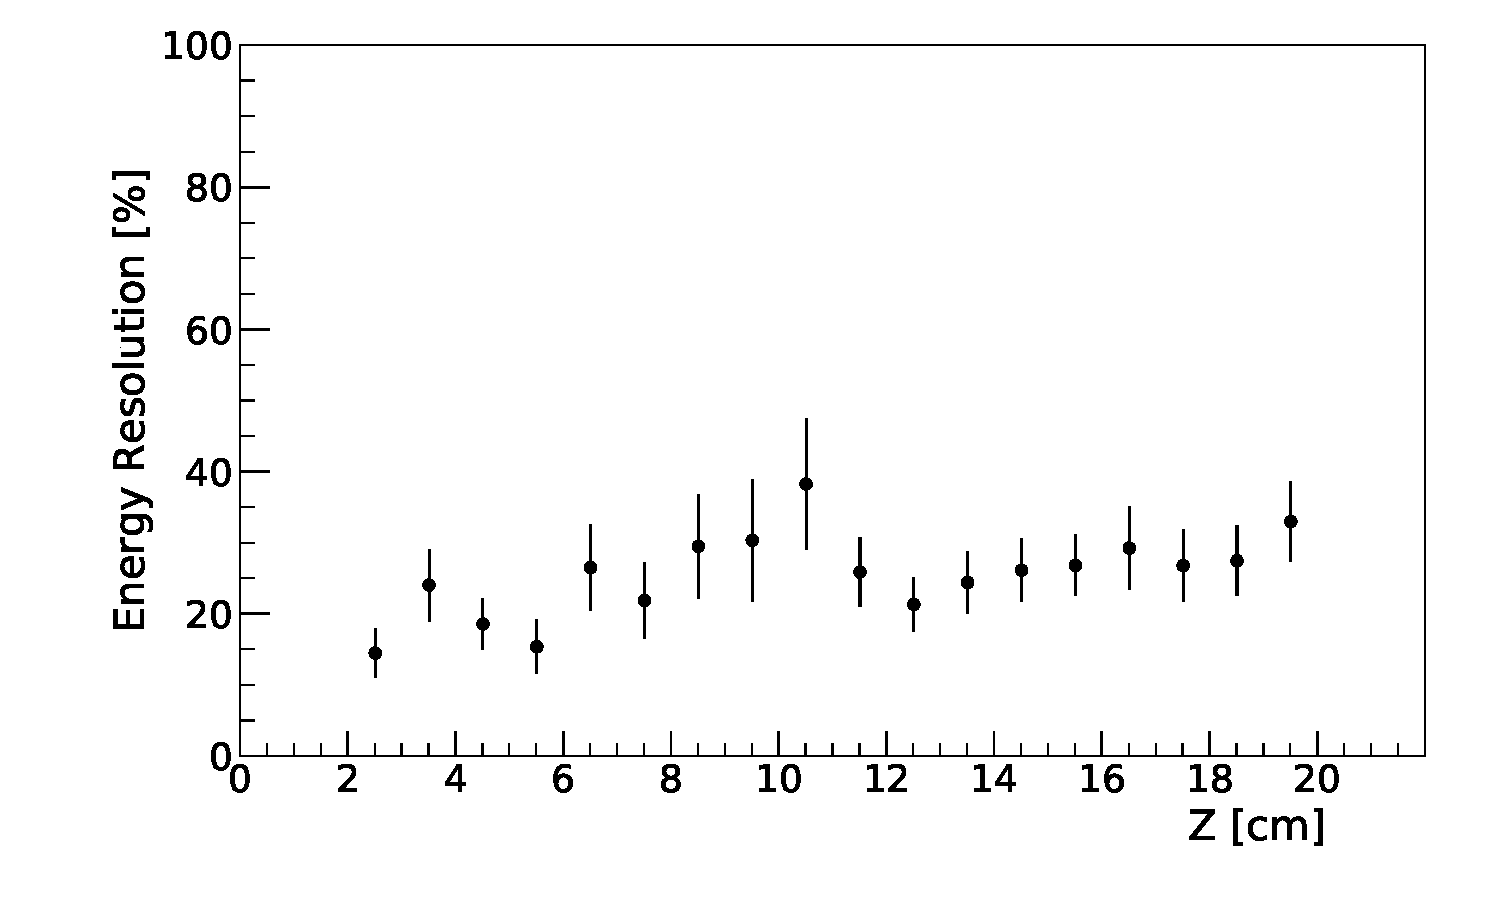
\includegraphics[width=3.4in]{Fig7-EnergyResultion-Z.pdf}
%\DeclareGraphicsExtensions.
\caption{Energy Resolution: standard deviation of total light yield  per track divided by its average as a function of the track $Z$ position.}
\label{fig:energyresvsZ}
\end{figure}

 The tracks can be divided in 36 portions of about 7 mm long - which are segments belonging to  the same  track. We evaluate the performance of LEMOn in  measuring their  position in space. An average energy loss of about 1.5 keV corresponds to each segment:  this allows to study the performance of LEMOn to tiny energy release and  - in perspective -  to predict  a very small energy threshold for the DM detection application.
 
  Among these 36 segments only 18 segments are retained in the central region of the field cage ellipse. This is due to the circumstance that an electric field distortion has been observed in regions close to the field cage rings, because of their different shape with respect to the GEM, in other LEMOn data~\cite{Costa:2019tnu}.
  
  Also the transverse  light profile of each segment can be described by  a Gaussian distribution. The fitted mean value  $Y_{mean}$ of this distribution  is used to identify the segment's $Y$ position. In Fig. \ref{fig:tracking}   examples of longitudinal and transverse light profiles are shown. 
  %Then, a linear fit to the 18 segments $Y_{mean}$ is performed (Fig. \ref{fig:tracking}). 
  The residual distribution of the 18 segments $Y_{mean}$ with respect to line obtained with HT is then  obtained. The standard deviation of this distribution evaluated in a sample of several tracks represents an estimate of the resolution on the segment's $Y$ position. This procedure is repeated for several images acquired with the BTF electrons  crossing the LEMOn field cage at different $Z$ positions (Fig.\ref{fig:XYres}).
The  dependence of the segment's $Y$ position resolution  on the $Z$ track coordinate is then interpolated with a linear function (Fig.\ref{fig:XYres}). While the best (extrapolated) resolution  of 83 $\pm$ 12 $\mu$m is obtained close to the GEMs ($Z$ = 0), we observe its worsening for larger $Z$: this is mainly due to the reduction of electrons for larger $Z$ that, besides reducing the produced light, also amplifies the effect of diffusion.


\begin{figure}[!ht]
\centering
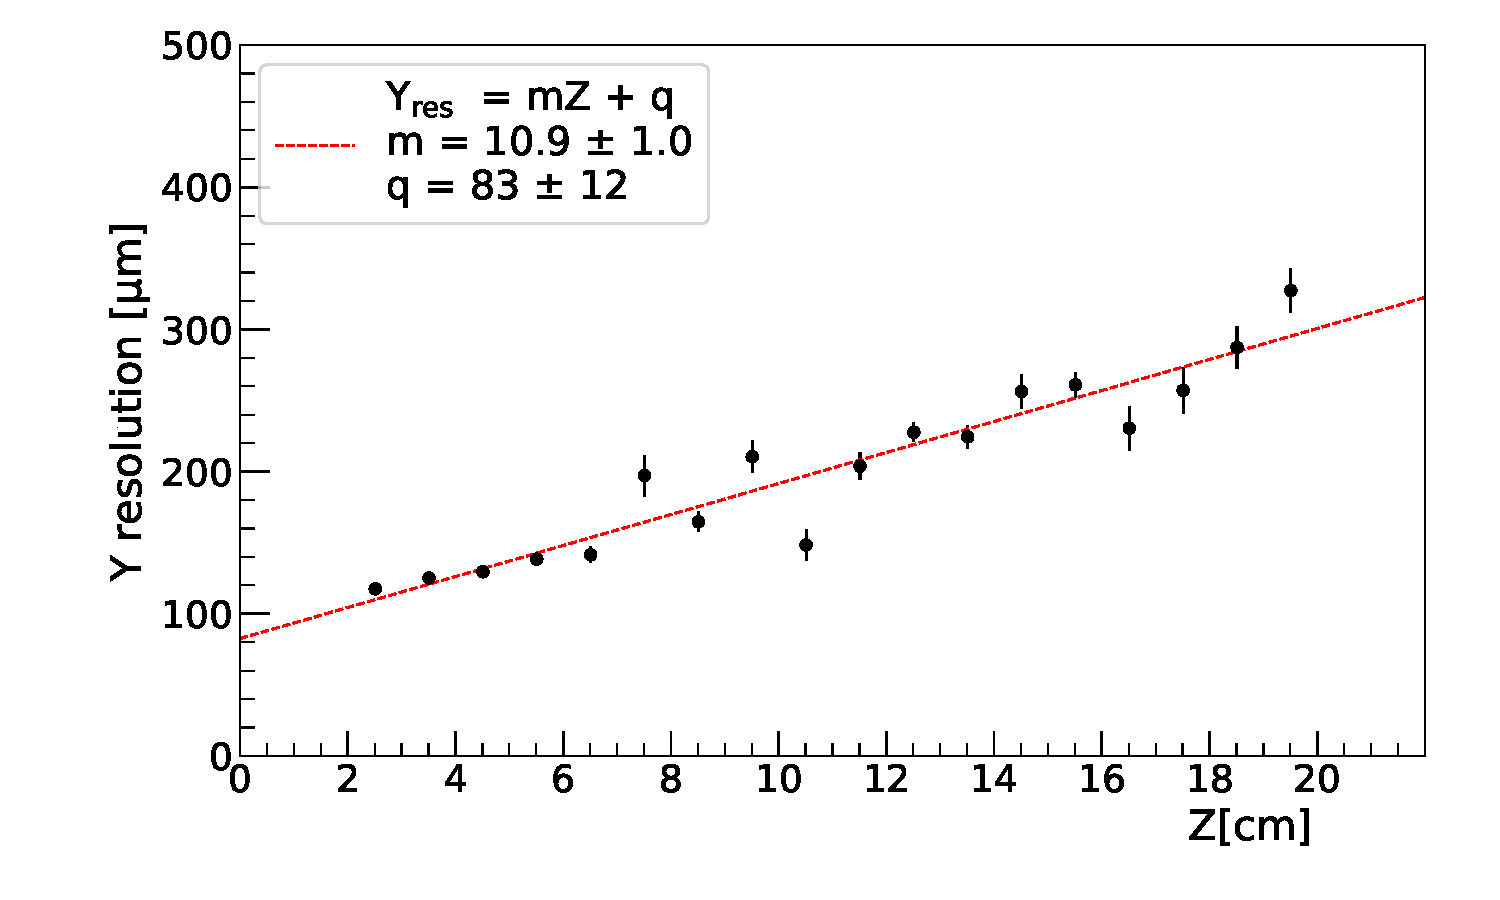
\includegraphics[width=3.4in]{Fig8-Resolution-Z.pdf}\DeclareGraphicsExtensions.
\caption{ Segment $Y$ position resolution  as a function of the track's $Z$ coordinate.}
\label{fig:XYres}
\end{figure}



\subsection{$Z$ coordinate measurement}

 While the ionization electrons are drifting  in the gas, they are  subject to a longitudinal and transverse diffusion. Their arrival $X$ and $Y$ coordinates and their arrival time at the GEMs are correlated with  their  production point position. The standard deviations of the position at the anode, $\sigma_X$  and $\sigma_Y$ are equal to $\sqrt{\frac{2DZ}{\mu E}}$ where $D$ is the diffusion coefficient, $\mu$ the electron mobility and $E$ the drift electric field \cite{bib:rolandiblum}. Moreover, during the avalanche formation within the GEMs a further diffusion of the avalanche electrons is taking place. Eventually, the light recorded from the sCMOS camera and PMT is related to the original point and time with an uncertainty that is larger for  production points farther in $Z$ from the GEMs.
  This is reflected in the transverse ($Y$) light distribution of each segment of the track: the     $\sigma_Y$  obtained from  the  Gaussian fit is in fact increasing with $\sqrt{Z}$. Therefore,  the segment's original $Z$ can be deduced by measuring  $\sigma$(Fig.\ref{fig:Diffusion}).
  
  \begin{figure}[!ht]
\centering
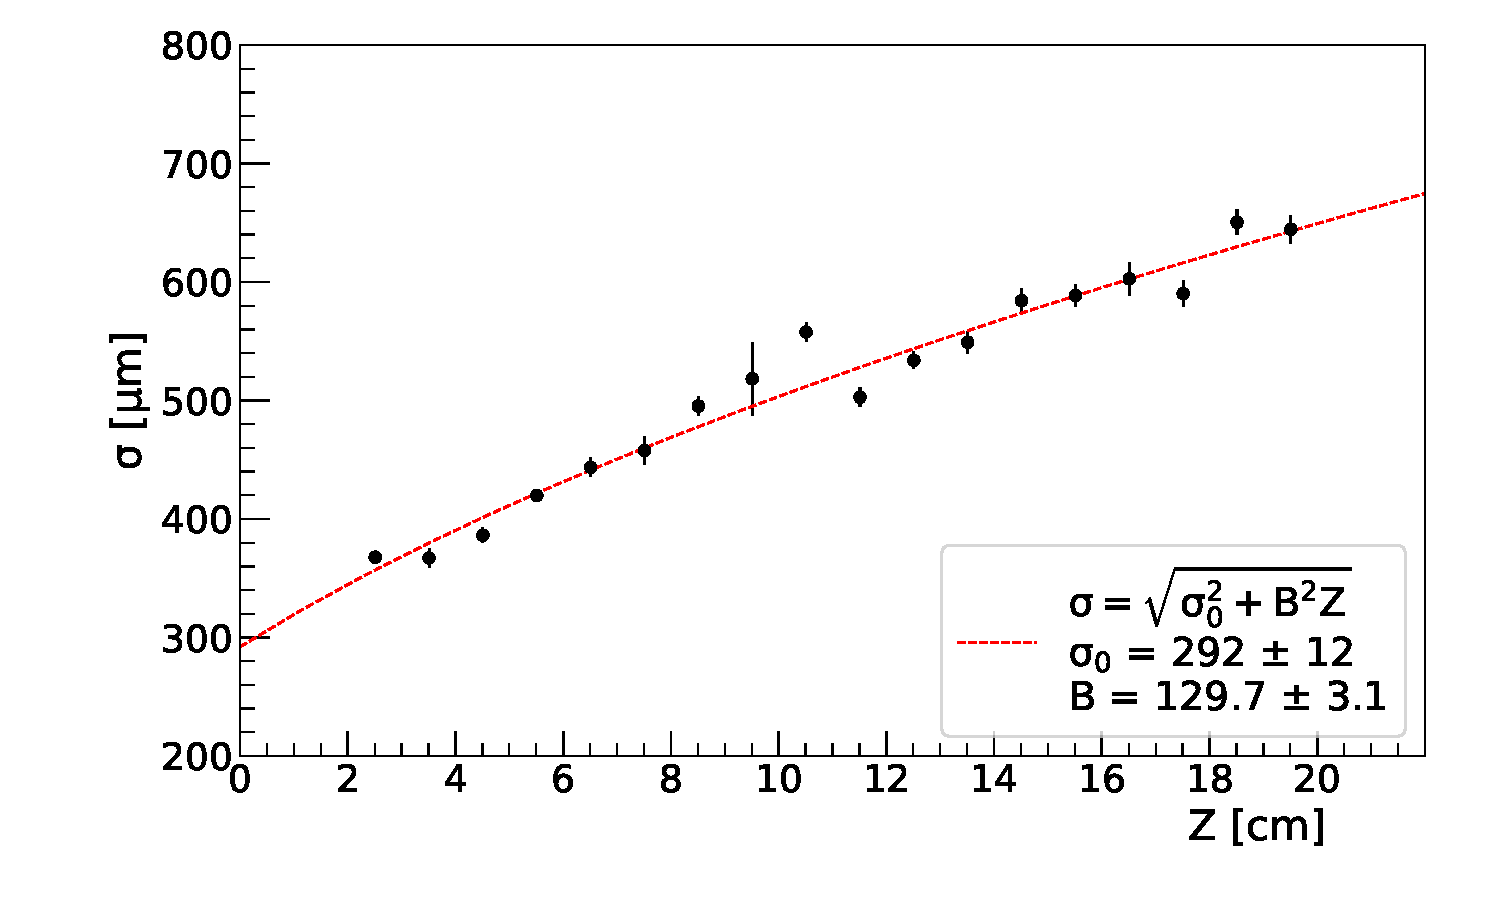
\includegraphics[width=3.4in]{Fig9-Diffusion-Z.pdf}\DeclareGraphicsExtensions.
\caption{ Average $\sigma$ of transverse light distribution for track segments as a function of the track $Z $ coordinate. }
\label{fig:Diffusion}
\end{figure}

 The observed values of  $\sigma$  are related to the track's $Z$  by  $\sigma = \sqrt{\sigma_0^2 + B^2 Z }$ 
 
 The transverse  diffusion coefficient $B$ in the gas is measured to be $129.7 \pm 3.1$ $\frac{\mu m}{\sqrt{cm}}$,  well in agreement with the expected value obtained with Garfield simulation (130 $\frac{\mu m}{\sqrt{cm}}$).

 The intercept at zero $\sigma_0$ =  $292 \pm 12$ $\mu$m is due to the contribution of the electron avalanche  propagation in the GEM stack, and it is  also well  in agreement with  simulations. 
 
From the same Gaussian fit to the light  $Y$ distribution of each segment, the amplitude $A$ can be obtained. Since $\sigma A$ is proportional to the total light $I$ of the segment we can  define $\eta = \frac{\sigma}{A}$ that is therefore  proportional to $\frac{\sigma_0^2 + B^2 Z}{I}$.

In Fig.~\ref{fig:etavsZ} we show the dependence of $\eta$ on the track's $Z$ coordinate. A quadratic fit gives a better representation of the data. This can be understood since in our data   the light $I$ shows a  linear decrease with $Z$ (see Fig.\ref{fig:lightvsZ}).
\begin{figure}[ht]
\centering
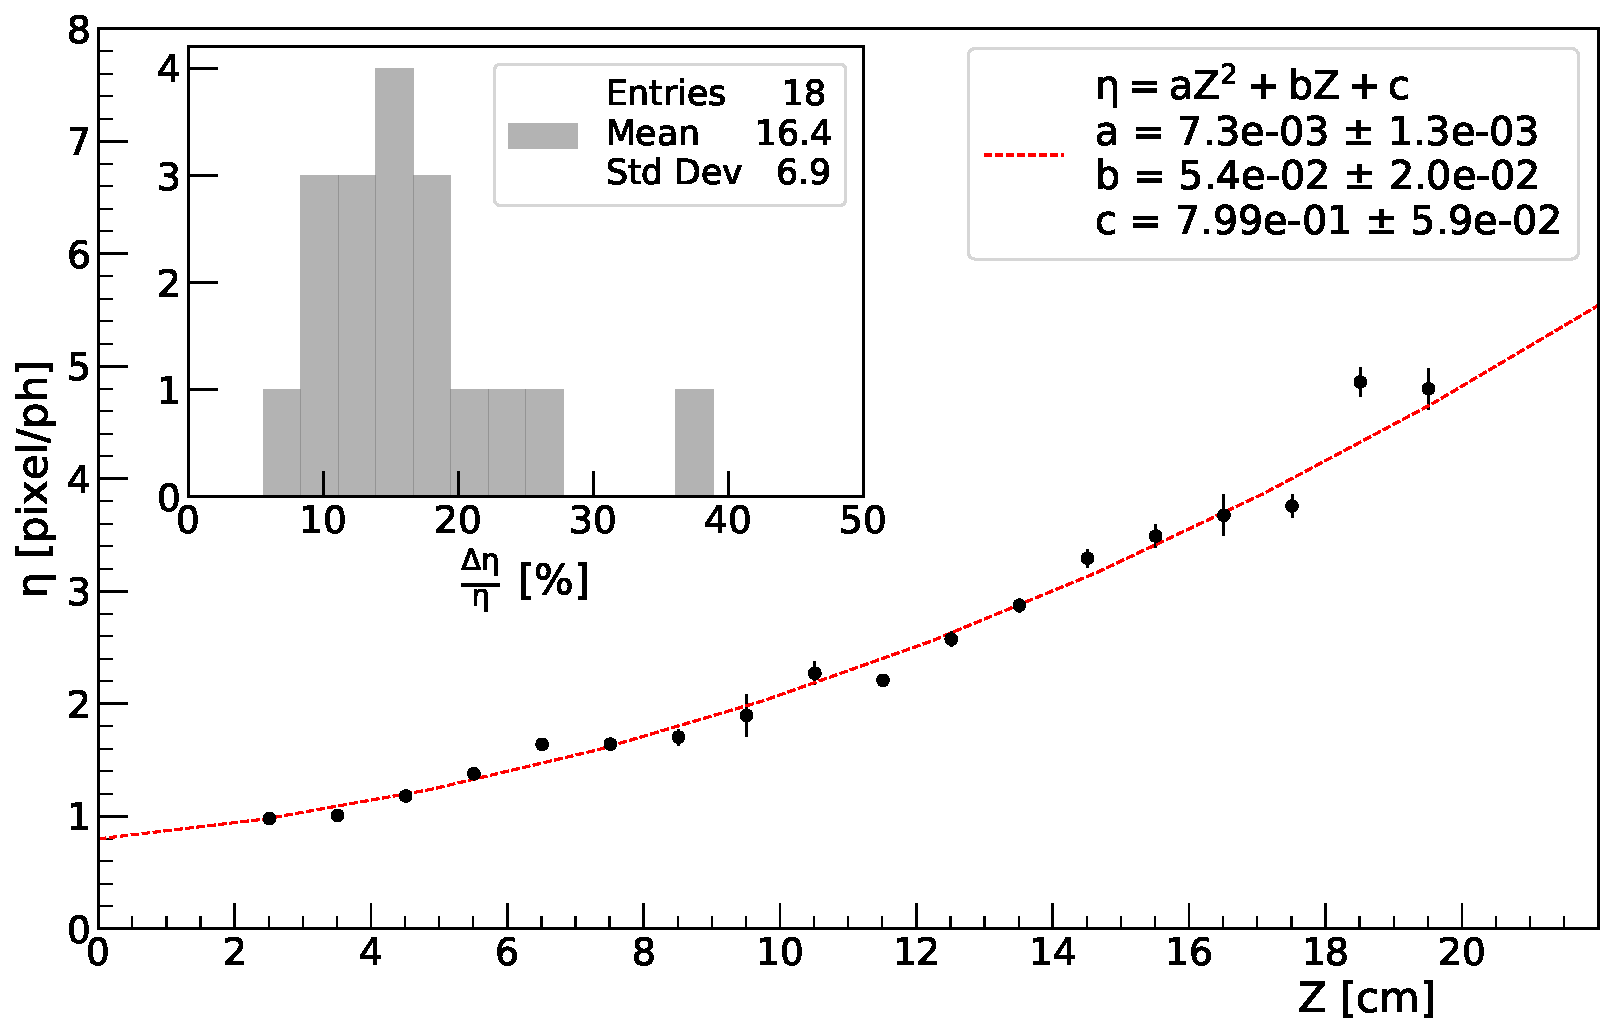
\includegraphics[width=3.1in]{Fig10-eta-CMOS-Z.pdf}\DeclareGraphicsExtensions.
\caption{ Average $\eta$  as a function of the track's $Z$ coordinated with a quadratic fit superimposed. Relative uncertainty on $\eta$ (inset) for the various $Z$ positions. }
\label{fig:etavsZ}
\end{figure}

A similar parameter $\eta_{PMT}$ can be defined from the analysis of the PMT waveform. In this case the total light of the track is recorded and we use the Pb-glass calorimeter signal of the BTF line to reject  events with  more than one  track. 
The amplitude of the  PMT waveform and its width can be similarly  used to calculate $\eta_{PMT}$. In this case the width of the waveform is larger for more distant tracks (larger $Z$)  due to the longitudinal diffusion of the drifting ionization electrons. By using the drift velocity, $\eta_{PMT}$ can be related to $Z$ similarly to $\eta$ (Fig.\ref{fig:Tdiffusion}).

\begin{figure}[ht]
\centering
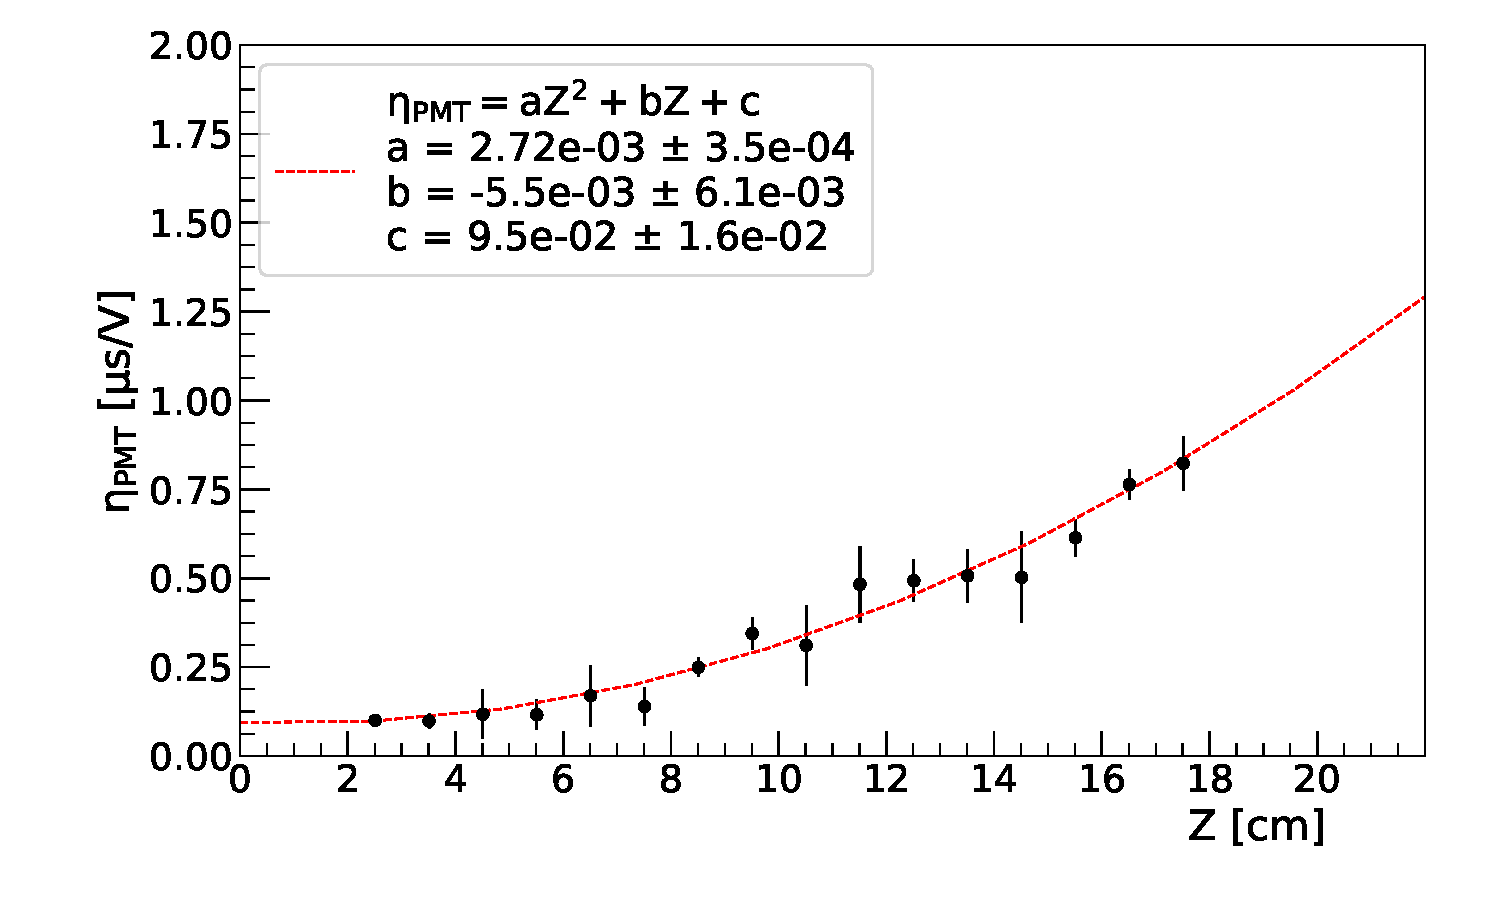
\includegraphics[width=3.4in]{Fig11-eta-PMT-Z.pdf}\DeclareGraphicsExtensions.
\caption{Average $\eta_{PMT}$ as a function of the track $Z$ coordinate. Data were not recorded for the largest $Z$ point since the beam was adding extra noise in the PMT.}
\label{fig:Tdiffusion}
\end{figure}


Transverse  and longitudinal  diffusion can therefore  be exploited to measure the longitudinal $Z$ coordinates. We can estimate $\frac{\Delta \eta}{\eta}$  from the standard deviation of the distributions of the  $\eta$ values. Since $\frac{\Delta \eta}{\eta} =\frac{\Delta Z}{Z} $  an estimate for  $\frac{\Delta Z}{Z}$  turns to be  in the range 10\% - 20\%.  


Therefore, a combination of the $\eta$ parameters would be very  useful to define a fiducial region  of a DM detector. Anode where the GEMs are located (at $Z$ $\sim$ 0 in LEMOn) and cathode  (at $Z$ $\sim$ 20 cm in LEMOn) are usually  the most radioactive elements in a DM detector. They are in fact sources of spurious nuclear recoils that would be easily  removed if  their $Z$ coordinate is measured.

\section{Conclusion}

The data collected at the Frascati Beam Test Facility with the LEMOn prototype, part of the CYGNO project, are confirming the potentiality of large optically readout  TPC  as detector for rare and low energy events. 

In this paper we have reported how  ultra-relativistic electron tracks can be  very efficiently reconstructed by collecting the light emitted from GEMs with a high resolution and high sensitivity sCMOS camera and a PMT.
 The analysis of the 7 mm long  segment of an electron track shows a  good spatial  and  energy resolution,  making  very promising the use of this  gas TPC down to few keV energy releases. Also a method based on the ionization electron diffusion can be very effective in determining  the segment's longitudinal position within the field cage. 
  This technology looks therefore extremely interesting in the development of a larger scale detector aiming to observe very rare processes as DM or Solar Neutrinos.
  

\section*{Acknowledgment}
A special thanks goes to M. Iannarelli, now retired, who assembled LEMOn and we are grateful to the BTF staff for the excellent and stable beam condition and their inexhaustible support.

This work was partially supported by the European Research Council (ERC) under the European Union’s Horizon 2020 research and innovation program (grant agreement No 818744).

Data available on request from the authors.



\nocite{*}
\bibliography{aipsamp}% Produces the bibliography via BibTeX.
\end{document}
%
% ****** End of file aipsamp.tex ******